% -*- root: ../../../main.tex -*-
\subsection{Safety e Consistency}
Nelle sezioni precedenti è stato descritto il funzionamento generale di RAFT includendo alcune proprietà e vincoli essenziali per mantenere consistenza tra i log durante le principali operazioni.\\
Qui di seguito ricordiamo le proprietà nominate nelle sezioni precedenti:

\begin{itemize}
	\item{\textbf{Election Safety:}} 
  Per un dato term è possibile al più eleggere \textbf{un solo leader}.
	La dimostrazione di questa proprietà è già stata discussa precedentemente nella sezione \ref{electionsaf} alla pagina \pageref{electionsaf}.
	\item{\textbf{Leader Append-Only:}}
  Il leader non cancella \textbf{mai}, ne sovrascrive le entry del proprio log.
  La proprietà è descritta in dettaglio nella sezione \ref{Log Replication}.
	\item{\textbf{Log Matching:}}
  La proprietà di log matching garantisce che:
	\begin{itemize}
		\item{\emph{Se due log hanno un entry con lo stesso index e stesso term, allora quell'entry contiene lo stesso comando(sono identiche)}}.
		\item{\emph{Se due \textit{entry} in log diversi hanno lo stesso index e lo stesso term, allora anche tutte le loro precedenti entry sono identiche tra i due log}}.
	\end{itemize}
	La proprietà è descritta in dettaglio nella sezione \ref{Log Replication} e nelle figure  \ref{fig:figure6} e \ref{fig:figure7}.
\end{itemize}
L'elenco sovrastante non è però completo! Attualmente ci sono casi che non sono gestiti e che possono causare notevole \textbf{inconsistenza} tra i log.
Ad esempio se il leader \textit{valida} alcune \textit{entry} mentre un dato follower è offline, nel caso in cui il follower venisse eletto esso potrebbe sovrascrivere le entry gia eseguite con quelle presenti nel proprio log.\\
E' necessario dunque completare l'algoritmo aggiungendo la proprietà chiave di tutte le state machine, la \textbf{State Machine Safety} property. 

  \paragraph{State Machine Safety}
  \emph{Non appena una entry è stata committata ed eseguita in una state machine, allora nessun altra state machine può committare una valore differente per la stessa entry}.



  \subsubsection{Election restriction}
  Durante le elezioni ci sono casi in cui non è possibile determinare se un \textit{entry} è committed oppure no.
  Come si può vedere in figura \ref{fig:figure 8} non è possibile determinare se l'ultima \textit{entry} è stata committed: per questo si aggiunge un ulteriore vincolo all'elezione di un candidate.
  Si restringere il range di elezione ai \textbf{Candidate} con il log più completo; questo per eleggere in ogni \textit{term} il migior \textbf{Candidate} quello che ha la visione più completa della situazione. 
  Come già detto un candidate invia ad ogni elezione le informazioni riguardanti il log.
  Più precisamente il \textbf{Candidate} invia solo le informazioni sull'ultima entry, l'\textit{index} e il \textit{term}, dato che queste informazioni definisco interamente il \textit{log}.
  \\
  Il criterio con cui viene fatta questa valutazione è il seguente: se l'ultimo term del log di V (votante) è maggiore di quello del log di C (candidato), allora la  richiesta viene rifiutata. Se invece i due ultimi term si equivalgono, la valutazione viene fatta tenendo conto della lunghezza del log. Se l'ultimo indice del log di C è maggiore di quello di V la richiesta viene accettata, altrimenti viene rifiutata.
  	
  \begin{figure}[H]
  	\centering
  	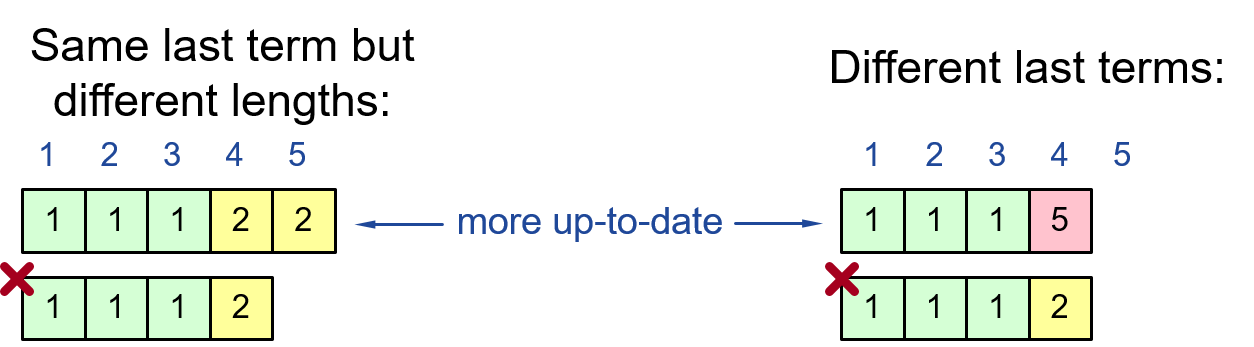
\includegraphics[width=0.99\columnwidth]{raft/pickingUpToDateLeader}
  	\captionsetup{singlelinecheck=off}
  	\caption[stateDiagramCaption]{
	In questo caso non è possibile determinare se l'ultima \textit{entry} è validata, inoltre solo il primo server può essere eletto dato che il terzo non è disponibile.}
  	\label{fig:figure8}
  \end{figure}
  \subsubsection{Committing entries from previous terms}
  \subsubsection{Neutralize Old Leaders}
  \subsubsection{Follower and Candidate Crash}
  \subsubsection{Timing and Availability}